\chapter{Jogo \textit{Color Clutter}}
\label{cap:color-clutter}

Dado que o módulo \textit{Speech to Text} está agora pronto, desenvolveremos um pequeno jogo com ele através do editor \textit{Godot} para demonstrar seu uso e analisar a qualidade do reconhecimento de voz na prática.

Ao longo deste capítulo, relatamos os passos realizados na criação do jogo \textit{Color Clutter}. Para melhor aproveitamento, o leitor precisará do editor \textit{Godot}, na versão 2.1.4, com o módulo instalado. Mencionamos, na seção \ref{modulePublishing}, alguns \textit{links} para baixar uma versão já pronta e para obter instruções de como compilar \textit{Speech to Text} com a \textit{game engine}.

% ---------------------------------------------------------------------

\section{Uso do editor \textit{Godot}}

Antes de começarmos o desenvolvimento do jogo, iremos descrever alguns elementos da interface do editor \textit{Godot} para melhor familiarizar o leitor com esta ferramenta.

% ---------------------------------------------------------------------

\subsection{Gerenciamento de projetos}

Ao executar o editor \textit{Godot}, o leitor é confrontado com a tela apresentada na figura \ref{editor-project-select}, na qual pode gerenciar seus projetos (jogos).

\begin{figure}[H]
  \centering
  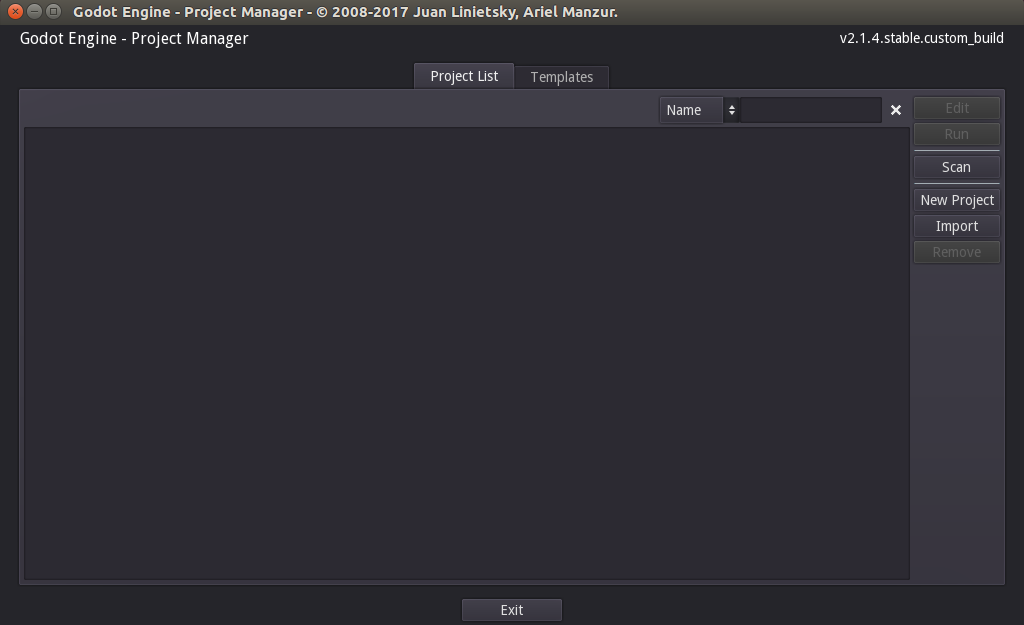
\includegraphics[width=.85\textwidth]{image/editor-project-select}
  \caption{Gerenciamento de projetos no editor \textit{Godot}}
  \label{editor-project-select}
\end{figure}

Projetos são listados na aba \textit{Project List}, onde podem ser abertos para edição ou removidos. Também é possível criar um novo jogo ou a importar um já existente. A criação de um projeto, por exemplo, é feita pelo botão \textit{New Project} e requer a especificação do caminho na qual será criado (\textit{Project Path}) e seu nome (\textit{Project Name}). Já a importação exige que o usuário escolha um caminho que contenha o arquivo \texttt{engine.cfg}, responsável por definir o diretório raiz do jogo.

Na figura \ref{editor-project-create}, exemplificamos a criação do projeto \textbf{teste} no diretório \texttt{\textasciitilde/Desktop/teste}. Ao clicar no botão \textit{Create}, o projeto é criado e o usuário é automaticamente encaminhado para a tela de edição de \textbf{teste}.

\begin{figure}[H]
  \centering
  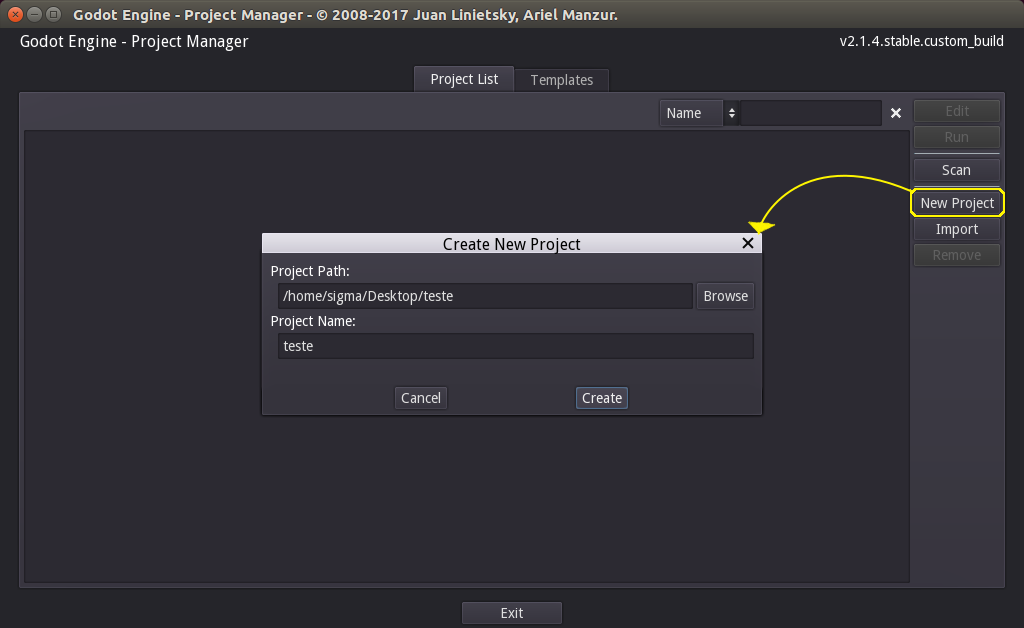
\includegraphics[width=.85\textwidth]{image/editor-project-create-edit}
  \caption{Criação do projeto \textbf{teste} no editor \textit{Godot}}
  \label{editor-project-create}
\end{figure}

% ---------------------------------------------------------------------

\subsection{Interface de edição de um projeto}

A criação de um novo projeto leva o usuário ao editor do mesmo. Continuando com nosso exemplo \textbf{teste}, sua tela de edição é apresentada na figura \ref{in-game-editor}.

\begin{figure}[H]
  \centering
  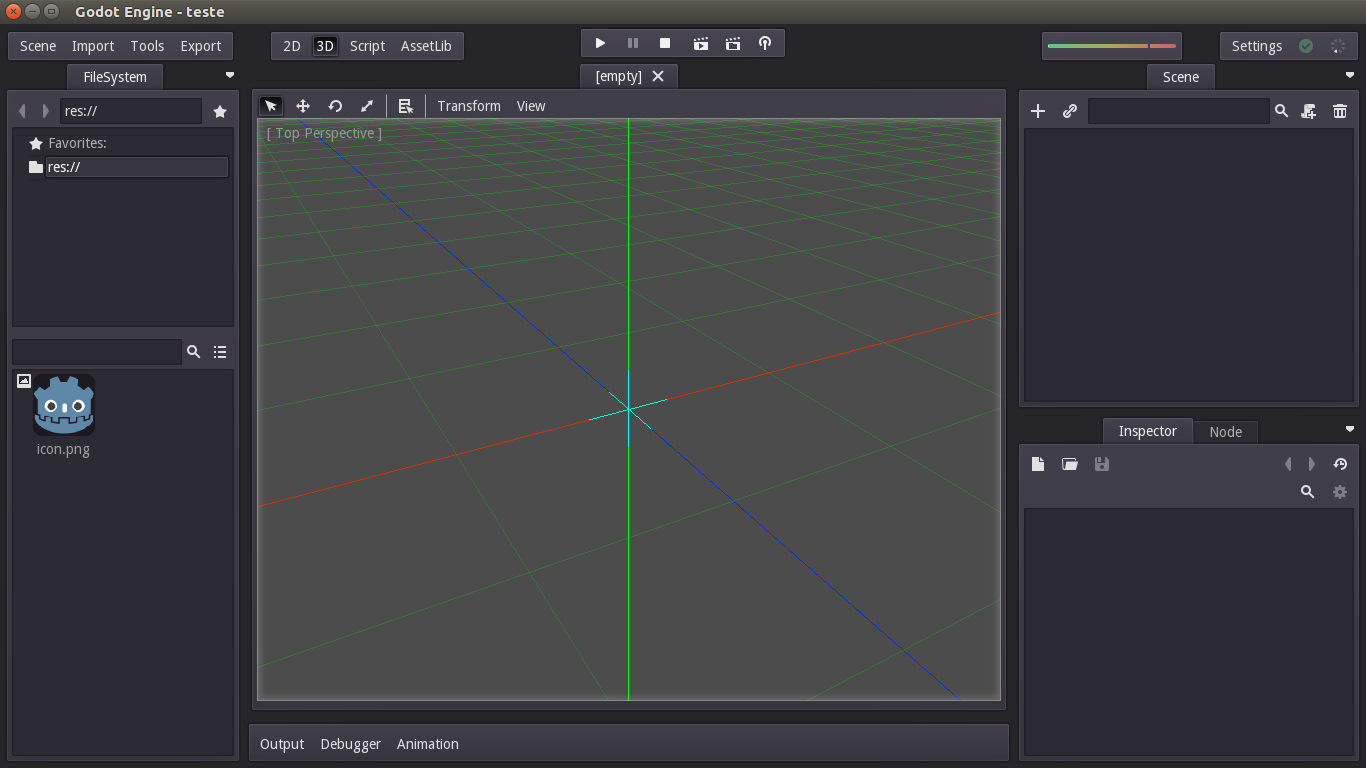
\includegraphics[width=.9\textwidth]{image/in-game-editor}
  \caption{Editor de um projeto \textit{Godot} (neste caso, \textbf{teste})}
  \label{in-game-editor}
\end{figure}

Uma explicação detalhada de todas as funcionalidades do editor fugiria do tema deste trabalho. Iremos, portanto, nos atentar às ferramentas principais, apresentadas a seguir.

% ---------------------------------------------------------------------

\subsection{Uso de \textit{nodes} e \textit{scenes}}

No canto superior direito do editor (conforme a figura \ref{in-game-editor}, a \textit{scene} (explicada na seção \ref{godotScene}) atual do projeto é indicada na aba de mesmo nome. É neste espaço que a hierarquia de \textit{nodes} (definidos na seção \ref{godotNode} pertencentes a esta cena é apresentada.

A criação de um \textit{node} para a cena é feita através do símbolo \textbf{\texttt{+}} desta aba, que leva o usuário a uma lista de nós existentes (figura \ref{editor-node}). Por curiosidade, recomenda-se que o leitor procure o nó \textbf{\textit{STTRunner}} (descrito na seção \ref{stt-runner}), fornecido pelo módulo \textit{Speech to Text}.

\begin{figure}[H]
  \centering
  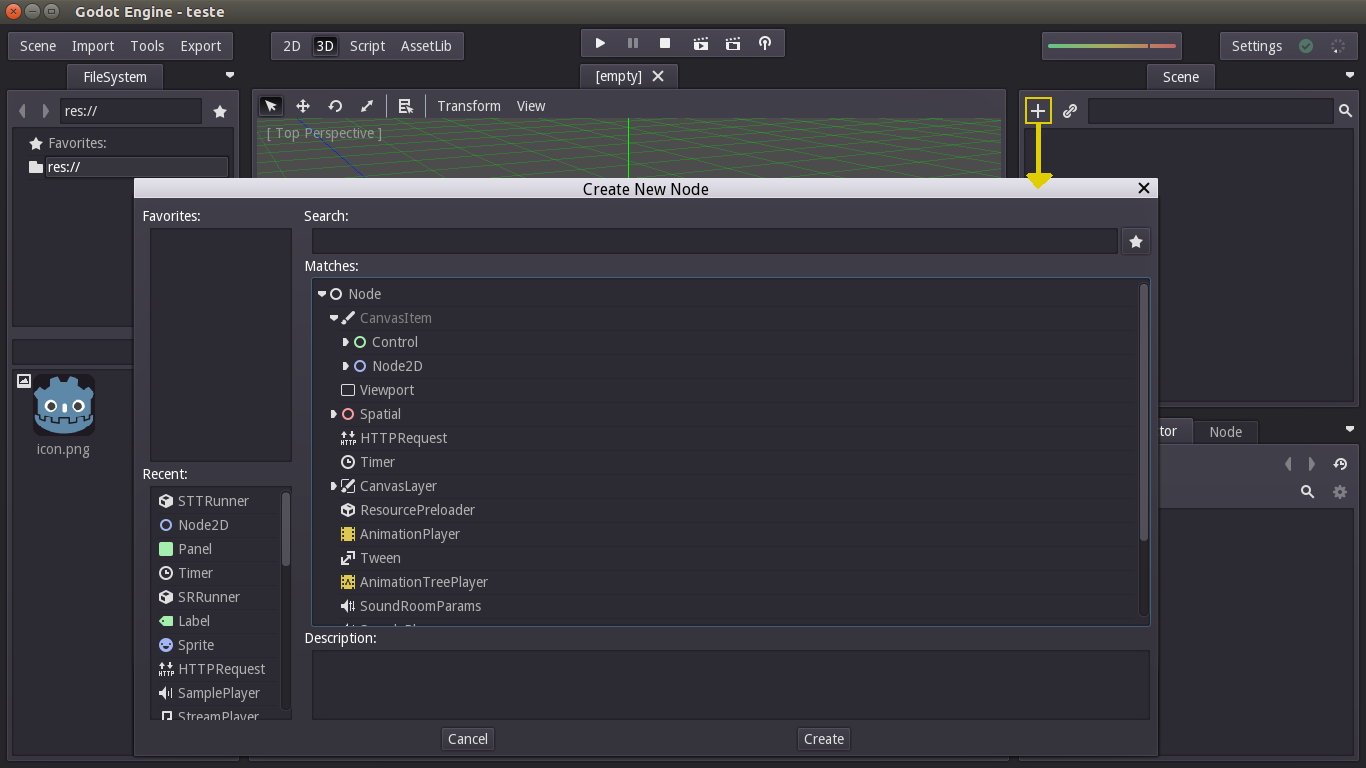
\includegraphics[width=.9\textwidth]{image/editor-node-edit}
  \caption{Lista de \textit{nodes} disponíveis no editor do projeto}
  \label{editor-node}
\end{figure}

Como exemplo, escolheremos, nesta lista, o \textit{node} \textbf{\textit{Label}} para representar um texto. A aba \textit{Scene} mostrará que foi adicionada à cena. Além disso, se selecionarmos este nó, a aba debaixo, \textit{Inspector}, indicará quais as suas propriedades editáveis, enquanto a janela central do editor mostrará seu posicionamento em relação a outros elementos do jogo (figura \ref{editor-label}).

\begin{figure}[H]
  \centering
  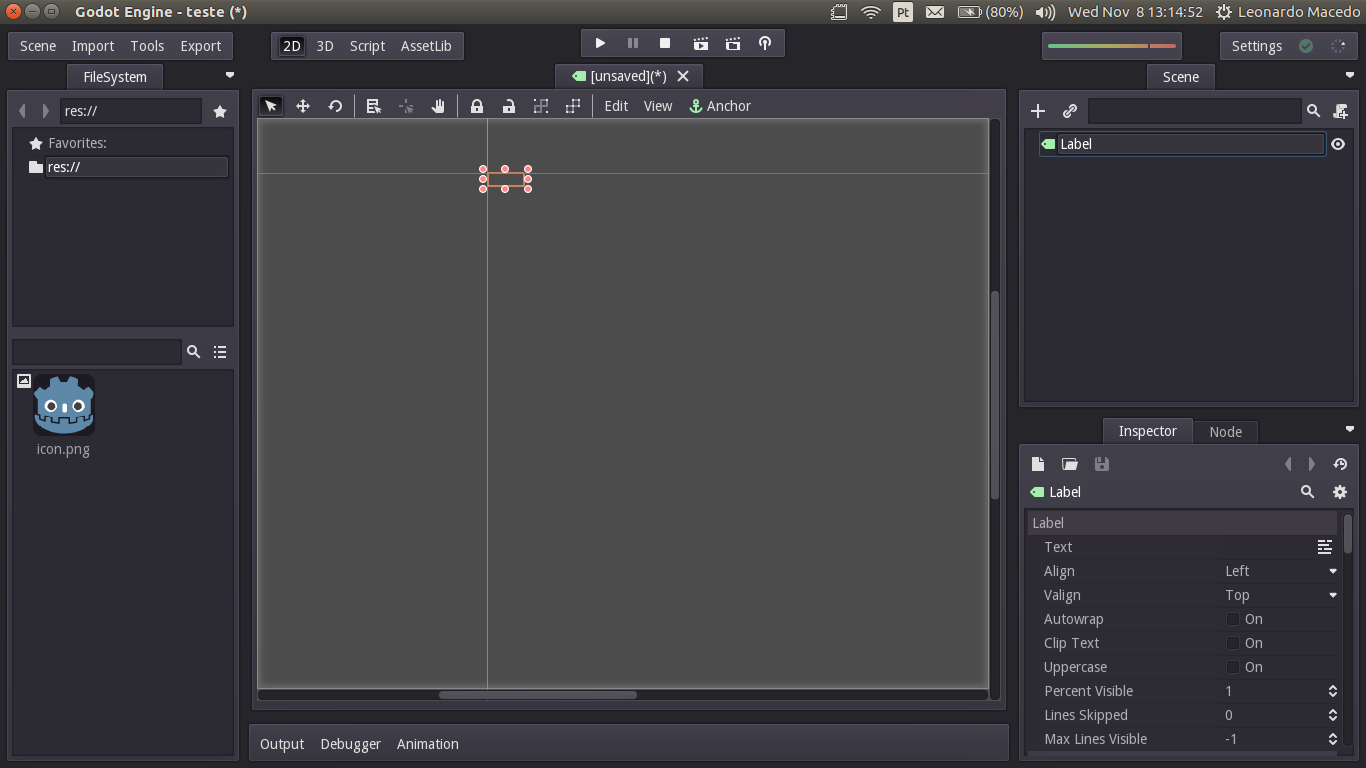
\includegraphics[width=.9\textwidth]{image/editor-label}
  \caption{Edição do \textit{node} \textbf{\textit{Label}}; note suas propriedadas na aba \textit{Inspector} (canto inferior direito)}
  \label{editor-label}
\end{figure}

Suponha que desejamos executar o jogo com apenas o nó \textit{Label}, com ele apresentando o texto \textit{``Hello World!''}. Para tanto, seguiremos os seguintes passos, ilustrados melhor pela figura \ref{editor-run-scene-edit}.

\begin{figure}[H]
  \centering
  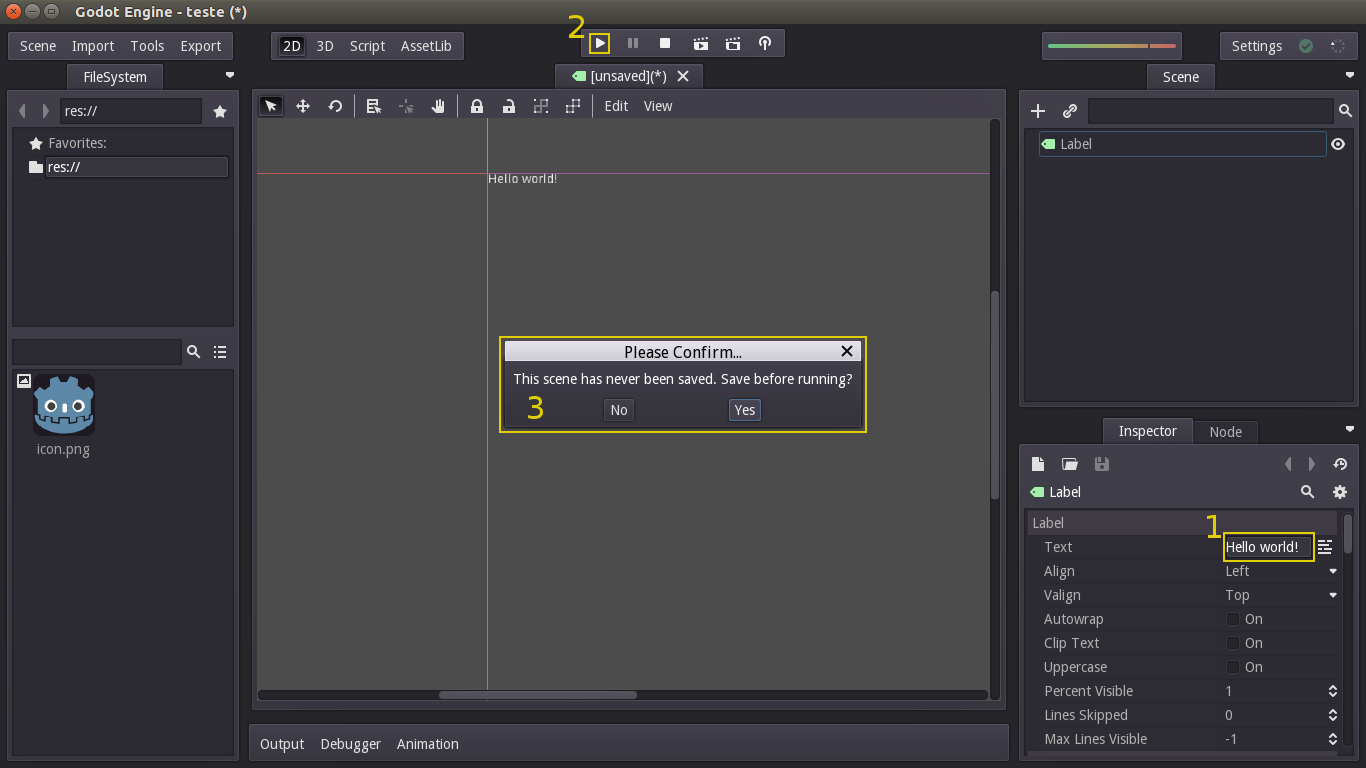
\includegraphics[width=.9\textwidth]{image/editor-run-scene-edit}
  \caption{Passos para execução da \textit{scene} contendo um \textit{Label} escrito \textit{``Hello World!''}}
  \label{editor-run-scene-edit}
\end{figure}

\begin{itemize}
\item Alterar o texto do \textit{Label} para \textit{``Hello World!''}. Isto é facilmente feito pela propriedade \textbf{\textit{Text}} na aba \textit{Inspector} (\textbf{1} na figura \ref{editor-run-scene-edit}).

\item Salvar a \textit{scene} atual. Uma forma de fazer isso para depois executar o jogo é clicar no botão \textit{Play the project} (triângulo no centro superior do editor; vide \textbf{2} na figura \ref{editor-run-scene-edit}). O editor apresentará uma janela para salvar a cena (\textbf{3} na figura \ref{editor-run-scene-edit}) como um arquivo cujo formato padrão é \texttt{.tscn}.

\item Se \textit{Play the project} foi usado para salvar a cena, imediatamente outra janela será exibida, solicitando a escolha da \textit{scene} a ser usada quando o jogo é iniciado. Basta escolher o arquivo \texttt{.tscn} que foi salvo no passo anterior.
\end{itemize}

O resultado, apresentado na figura \ref{editor-hello-world}, será a abertura de uma nova janela para a execução do jogo. Note o texto \textit{``Hello World!''} em seu canto superior esquerdo.

\begin{figure}[H]
  \centering
  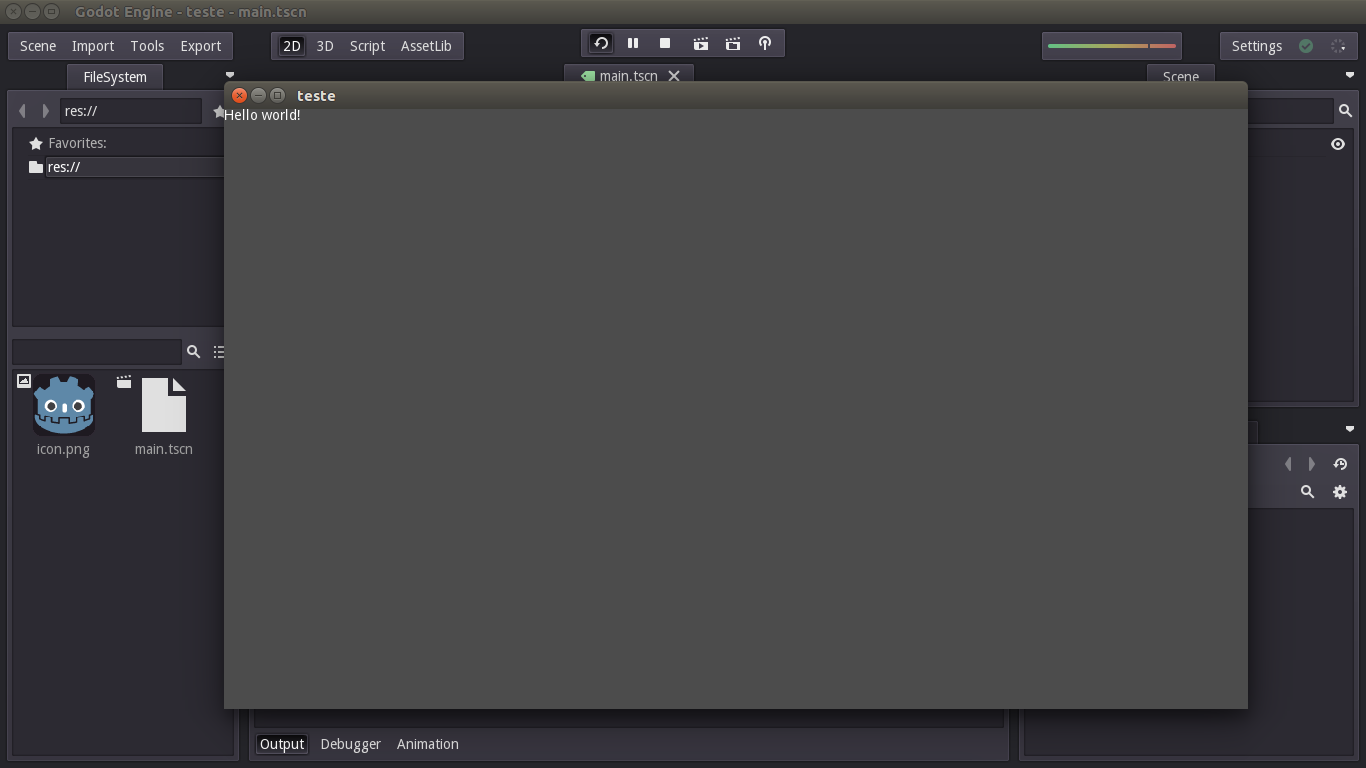
\includegraphics[width=.9\textwidth]{image/editor-hello-world}
  \caption{Execução da \textit{scene} contendo um \textit{Label} de texto \textit{``Hello world!''}}
  \label{editor-hello-world}
\end{figure}

% ---------------------------------------------------------------------

\subsection{Uso de \textit{GDScript}}

A linguagem \textit{GDScript} (introduzida na seção \ref{godotLanguages}) é usada para escrever trechos de código que definem o comportamento de \textit{nodes} \citep{godotScripting}.

Para adicionar um \textit{script} a um nó, basta clicar em seu nome, na aba \textit{Scene}, com o botão direito e escolher \textbf{\textit{Add Script}} (figura \ref{editor-attach-script}). Uma janela irá surgir, onde é necessário preencher apenas o campo \textit{Path} para definir o nome do \textit{script} (figura \ref{editor-script-window}).

\begin{figure}[H]
  \centering

  \begin{minipage}{.5\textwidth}
    \centering
    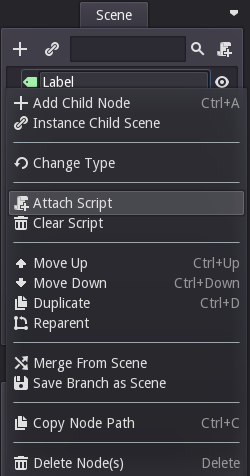
\includegraphics[width=.6\textwidth]{image/editor-attach-script}
    \caption{Opção \textbf{\textit{Attach Script}} para o \textit{node} \textit{Label}}
    \label{editor-attach-script}
  \end{minipage}%
  \begin{minipage}{.5\textwidth}
    \centering
    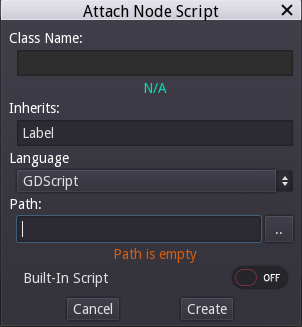
\includegraphics[width=.75\textwidth]{image/editor-script-window}
    \caption{Janela de criação do arquivo \textit{script}}
    \label{editor-script-window}
  \end{minipage}
\end{figure}

Suponha que definimos \textit{Path} como \texttt{res://script.gd} na figura \ref{editor-script-window}. Ao clicarmos em \textit{Create}, a aba central do editor mudará para \textbf{\textit{Script}}, onde o código do arquivo pode ser modificado. Ilustramos a modificação ocorrida na figura \ref{editor-script-write}. Por curiosidade, veja, neste mesma imagem, que todos os recursos (como \textit{scenes}, \textit{scripts} e gráficos) existentes dentro do diretório do projeto são mostrados no canto inferior esquerdo do editor.

\begin{figure}[H]
  \centering
  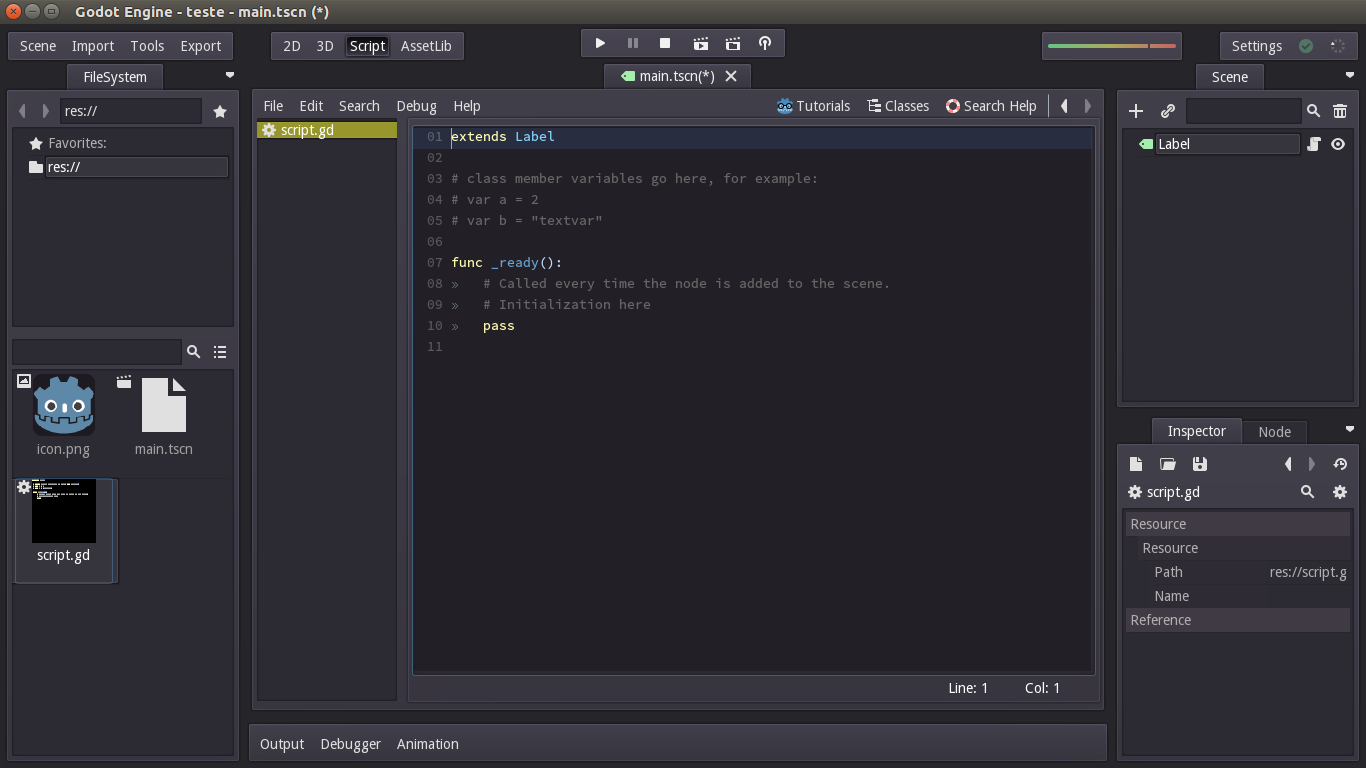
\includegraphics[width=.9\textwidth]{image/editor-script-write}
  \caption{A aba \textbf{\textit{Script}} permite modificar arquivos homônimos}
  \label{editor-script-write}
\end{figure}

Não iremos ensinar, neste trabalho, a linguagem \textit{GDScript} porque o ganho nisso seria mínimo. Um tutorial detalhado, apresentado por \textit{Godot} em \citep{godotGDScriptTutorial}, já existe com esta finalidade. No entanto, explicaremos duas funções predefinidas pela linguagem e que possuem bastante importância no controle de \textit{nodes}.

\subsubsection{\texttt{\_ready()}}

A função \texttt{\_ready()} é chamada sempre que o \textit{node} é adicionado à cena. É geralmente usada para inicializar atributos e preparar configurações de comportamento.

É importante lembrar que nós são organizados em árvore. Portanto, o \texttt{\_ready()} de um \textit{node} pai é sempre chamado antes da função respectiva nos filhos.

\subsubsection{\texttt{\_process(delta)}}

\texttt{\_process()} é uma função chamada repetidamente enquanto o nó existir na cena e \texttt{set\_process(true)} tiver sido chamada previamente (em \_ready(), por exemplo) para solicitar seu uso. Seu único argumento, \texttt{delta}, representa o tempo desde a última atualização de \textit{frame} do jogo.

Esta função é muito útil para executar trechos de código periodicamente durante um jogo. Por exemplo, imagine um jogo em que a personagem controlada pelo usuário possua um certo número de pontos de vida. Poderia-se utilizar \texttt{\_process()} para checar se este valor chegou a zero e, se afirmativo, alterar a \textit{scene} atual para a do fim de jogo.

% ---------------------------------------------------------------------

\section{Planejamento}

Além da escrita de código, jogos costumam usar diversos materiais, ou \emph{assets}, como modelos gráficos, música, sons, fontes e texturas. A criação destes demanda bastante tempo e em geral exige uma equipe diversificada e qualificada. Portanto, gostaríamos de produzir um jogo que utilize poucos \textit{assets}; buscaremos quaisquer materiais necessários em páginas Web que os disponibilizem para uso grátis e sem licença.

Quanto à jogabilidade, desejamos colocar ênfase na funcionalidade de reconhecimento de voz; este é o objetivo em sua criação, afinal. O uso de alguns poucos comandos orais em um jogo curto é o ideal para deixar as regras simples, mas com interação razoável com o usuário.

Por fim, definiremos que o jogo e reconhecimento de voz usarão \textbf{inglês americano} (\textit{US English}), pois sabemos que um modelo acústico e arquivo de dicionário para \textit{Pocketsphinx} existem e são de uso livre para esta língua.

Com estas características em mente, planejamos o jogo \textbf{\emph{Color Clutter}}.

% ---------------------------------------------------------------------

\subsection{Descrição de \textit{Color Clutter}}

Conforme o nome sugere, \textit{Color Clutter} é um jogo cuja temática envolve uma ``confusão'' entre cores.

Uma típica tela do jogo consiste em um fundo totalmente preenchido com alguma cor \(X\). Em alguma posição da tela, uma outra cor \(Y\) aparece escrita em um tom \(Z\). O objetivo do usuário é falar a cor correta (\(X\), \(Y\) ou \(Z\)), de acordo com o que é solicitado em uma legenda apresentada na tela.

Para acrescentar um aspecto competitivo e tornar \textit{Color Clutter} mais lúdico, o jogo será no formato de rodadas, onde marcaremos quantos acertos o usuário consegue em 1 minuto. Cada resposta correta altera aleatoriamente as cores e a posição da palavra na tela; não há penalidade para uma resposta errada, exceto a perda de tempo acarretada pela mesma.

A figura \ref{color-clutter-screen} apresenta a tela do jogo durante uma rodada. O canto superior esquerdo informa qual cor deve ser pronunciada, enquanto o canto superior direito exibem o tempo restante e o \textit{score} (pontuação) atual do jogador. Na situação apresentada, o usuário precisaria falar a cor correspondente ao \textit{background} (fundo): \textbf{\textit{blue}}.

\begin{figure}[H]
  \centering
  \includegraphics[width=.8\textwidth]{image/color-clutter-screen}
  \caption{Tela do jogo \textit{Color Clutter} durante uma rodada}
  \label{color-clutter-screen}
\end{figure}

% ---------------------------------------------------------------------

\section{Desenvolvimento}

A simplicidade de \textit{Color Clutter} nos levou a implementá-lo com apenas uma \textit{scene}. A árvore de \textit{nodes} que o compõe é apresentada na figura \ref{color-clutter-nodes}.

\begin{figure}[H]
  \centering
  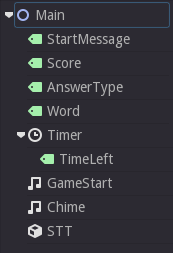
\includegraphics[width=.3\textwidth]{image/color-clutter-nodes}
  \caption{Árvore de \textit{nodes} utilizada em \textit{Color Clutter}}
  \label{color-clutter-nodes}
\end{figure}

Explicamos, a seguir, o funcionamento geral do jogo e detalhamos alguns dos textit{nodes} utilizados.

% ---------------------------------------------------------------------

\subsection{Máquina de estados}

Em termos de funcionamento geral, o jogo transita entre dois estados, \textit{Start} e \textit{Running}. O primeiro caso define o início do jogo, onde espera-se o usuário falar \textit{start} para começar uma partida. Ao reconhecer tal palavra, transita-se para o estado \textit{Running}, correspondente à partida em si, onde o usuário tem 1 minuto para acertar o máximo de cores possíveis. Terminado este tempo, exibe-se a pontuação do jogador e volta-se para o estado \textit{Start}.

A qualquer momento, o usuário pode sair do jogo através do comando de voz \textit{exit}, imediatamente finalizando \textit{Color Clutter}.

% ---------------------------------------------------------------------

\subsection{\textit{Node} \texttt{Main}}

\texttt{Main} é um \textit{Node2D}, que é um nó base para jogos em 2D; por isso seu uso como o \textit{node} raiz da cena.

Conforme indicado na figura \ref{color-clutter-nodes}, este nó contém \texttt{STT}, que é do tipo \textit{STTRunner}. Para poder utilizá-lo, \texttt{Main} prepara dois objetos em \texttt{\_ready()}:

\begin{itemize}
\item Um objeto da classe \textit{STTConfig} (explicado na seção \ref{stt-config}). Definiram-se os arquivos de configuração necessários: um modelo acústico em inglês, um dicionário de palavras em inglês e um arquivo de palavras-chave contendo os comandos usados no jogo. Neste último, os valores de limiar escolhidos foram, em geral, baseados no número de fonemas existentes no comando. Por fim, utilizou-se o método \texttt{init()} para inicializar a instância, deixando-a pronta para uso no \textit{STTRunner}.

\item Um objeto da classe \textit{STTQueue} (explicado na seção \ref{stt-queue}). Esta fila guarda os comandos de voz falados pelo usuário.
\end{itemize}

O laço geral do jogo (\textit{game loop}) está implementado na função \texttt{\_process(delta)}, que é apresentada em pseudocódigo a seguir:

\begin{algorithm}
\begin{algorithmic}[1]
\Function{}{} {\_process}(delta)
\If {\textbf{not} stt\_queue.empty()}
    \State {command $\leftarrow$ stt\_queue.get()}
\EndIf
\State
\If {game\_state == START}
    \If {command == "start"}
        \State {start\_game()}
    \EndIf
\ElsIf {game\_state == RUNNING}
    \If {command == right\_answer}
        \State {update\_score()}
        \State {update\_round()}
    \EndIf
\EndIf
\State
\If {command == "exit"}
    \State {exit\_game()}
\EndIf
\EndFunction
\end{algorithmic}
\end{algorithm}

A função \texttt{update\_score()} é responsável por atualizar a pontuação guardada no \textit{Label} \texttt{Score}, enquanto \texttt{update\_round()} altera os \textit{Labels} \texttt{Word} (a palavra-cor espalhada na tela) e \texttt{AnswerType} (que descreve se a próxima resposta é a palavra, sua cor ou o fundo).

% ---------------------------------------------------------------------

\subsection{\textit{Node} \texttt{Word}}

\texttt{Word} é um nó do tipo \textit{Label}, correspondendo à palavra gerada aleatoriamente pela tela. Quando o usuário acerta a cor da rodada, sua posição é alterada para algum valor dentro dos limites da tela. Garante-se que a cor em que \texttt{Word} é escrita não seja igual à cor de fundo (uma palavra azul em um fundo azul, por exemplo, seria de difícil visualização).

% ---------------------------------------------------------------------

\subsection{\textit{Node} \texttt{Timer}}

\texttt{Timer} é um nó de tipo homônimo. Como o nome indica, ela é usada como um relógio: após atribuir um valor de tempo e acioná-lo, o \textit{Timer} realizará realizar uma contagem regressiva, realizando automaticamente uma chamada de função (\textit{callback}) quando chegar a zero.

No contexto de \textit{Color Clutter}, este \textit{node} automaticamente atualiza seu filho \texttt{TimeLeft}, que é um \textit{Label} usado para indicar, na tela, o  tempo restante de jogo. \texttt{Timer} chama uma função em \texttt{Main} quando a partida acaba, com o objetivo de alterar o estado do jogo para \textit{Start}.

% ---------------------------------------------------------------------

\subsection{\textit{Nodes} \texttt{GameStart} e \texttt{Chime}}

\texttt{GameStart} e \texttt{Chime} são nós do tipo \textit{StreamPlayer}. Guardam um efeito sonoro tocado no início do jogo e quando o usuário acerta a cor, respectivamente.

% ---------------------------------------------------------------------

\section{Testes}

\textit{Color Clutter} foi testado por 10 pessoas com boa fluência em inglês. A maioria dos testadores utilizavam alguma versão de \textit{Windows} (versões 7, 8 ou 10), com três testes sendo feitos nas distribuições \textit{Ubuntu}, \textit{Debian} e \textit{Linux Mint} do sistema operacional \textit{Unix}.

Um dos primeiros resultados visualizados é que não houve diferença perceptível no reconhecimento de voz execução entre os sistemas operacionais. Todos os testadores comentaram que a velocidade de reconhecimento estava rápida (menos de 1 segundo).

No entanto, praticamente todas as pessoas envolvidas no teste comentaram que alguns comandos não eram reconhecidos na primeira vez em que eram pronunciados, exigindo-se repeti-los 2 ou 3 vezes até serem aceitos. Destacam-se as cores \textit{green}, \textit{orange} e \textit{purple} como as palavras que, em geral, geravam maior dificuldade de reconhecimento.

A efeito de comparação, executou-se uma API de reconhecimento de voz desenvolvida pelo Google \citep{googleSpeechAPI}, configurada para o inglês americano, simultaneamente em que \textit{Color Clutter} era jogado. Este programa reconheceu todas as palavras proferidas enquanto \textit{Color Clutter}, por vezes, não entendia algum comando. Duas respostas possíveis surgem para esta diferença: a eficiência da API do Google é bem maior do que a de \textit{Pocketsphinx}, ou é necessário um ajuste no limiar das palavras-chave do jogo (isto é, é possível que uma pronúncia muito parecida com a da fonética do dicionário esteja sendo exigida).

% ---------------------------------------------------------------------

\section{Divulgação}

Todo o código fonte do projeto \textit{Color Clutter} encontra-se em um repositório no GitHub do autor \citep{colorClutterGitHub}, juntamente com as instruções do jogo. Também foram disponibilizados binários para \textit{Windows} e \textit{Unix} \citep{colorClutterDownload}.

\textit{Color Clutter} foi divulgado nos mesmos dois fóruns de \textit{Godot} onde publicou-se sobre \textit{Speech to Text}:

\begin{itemize}
\item \textbf{Godot Engine Q\&A} \citep{colorClutterGodotQA}: Embora não seja mais voltado para tirar dúvidas, publicou-se o jogo no site oficial de \textit{Godot}.

\item \textbf{Godot Developers} \citep{colorClutterGodotDevelopers}: Voltado principalmente para jogos produzidos na \textit{game engine}.
\end{itemize}
